\documentclass[UTF8,a4paper]{paper}
\usepackage{ctex}
\usepackage{amsmath}
\usepackage{pdfpages}
\usepackage{graphicx}
\usepackage{wrapfig}
\usepackage{listings}
\usepackage{multicol}
\title{压控电阻的设计}
\author{张蔚桐\ 2015011493\ 自55}
\begin {document}
\newenvironment{figurehere}
{\def\@captype{figure}}
{}
\newcommand{\tabincell}[2]{\begin{tabular}{@{}#1@{}}#2\end{tabular}}
\maketitle
\tableofcontents
\clearpage
\section{引言}
根据查阅到的相关资料,目前的压控电阻往往采取AD/DA转换器设计,而由于相比于模拟元件来说,
数字元件往往造价较高,而且数——模转换过程中往往存在一些误差,而完全由模拟元件组成的电路少之又少,
因此设计一个完全由模拟元件组成的压控电阻成为了我研究的一个兴趣点。

在根据我们的了解,非线性元件,如JFET在其可变电阻区可以有$U_G$控制在$U_{DS}$间形成一个可变电阻,
然而这个压控电阻存在非线性,受外部电压影响较大等问题不能在实际中加以利用,因此,我们采取闭环反馈的方式,
试图设计一个大范围线性的可变电阻

\section{电路原理图}
电路原理图如图\ref{1}所示,整个电路在$V_C$的作用下表现为一个$U_i$端口对地的电阻。$V_C$和$U_i$对地电阻的关系
为$$R_{ui}=10V_C\mathrm{k}\Omega/\mathrm{V}$$

\begin{figure}
\centering
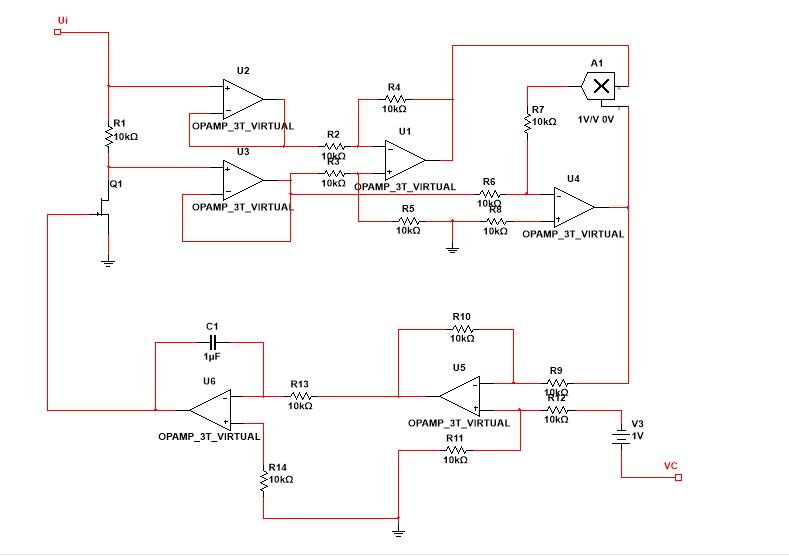
\includegraphics[width=\textwidth]{1.jpg}
\caption{电路原理图}
\label{1}
\end{figure}

根据电路原理图我们可以看出,被控对象为由$R_1=10\mathrm{k}\Omega$和JFET$Q_1$组成的串联支路,
集成运放$U_2,U_3$对电路进行阻抗变换之后相减,分别得到了$Q_1$上的分压$U_{Q_1}=-U_3$和$R_1$上的分压
$U_{R_1}=-U_1$其中$U_1,U_3$分别代表集成运放$U_1,U_3$的输出电压,经过有$U_4,A_1$组成的除法器之后,$U_4$
输出显然为$\frac{R_{Q_1}}{R_1}$,即可计算$Q_1$的实际电阻。

我们输入的控制电压$U_C$从图中VC引脚输入,$U_5$对实际的$Q_1$电阻和控制量相减,得到输出为
$U_5=U_C-1-\frac{R_{Q_1}}{R_1}$。

接下来解释$U_6$一阶积分环节的工作原理,根据之前的分析,我们假设目前$$U_5=U_C-1-\frac{R_{Q_1}}{R_1}>0$$
积分环节开始反向积分,使得$U_6$输出负电压,增大$R_{Q_1}$使得$U_5$减小。可以看出,电路直到$U_5$输出电压为0,
$U_6$给出一个稳定的$U_{gs}$电压时才可稳定。此时我们可以看出,$$U_C-1-\frac{R_{Q_1}}{R_1}=0$$ $$R_{Q_1}
=R_1(U_C-1)$$而整个受控电路由$Q_1$和$R_1$串联,立即得到$$R=R_1U_C=10V_C\mathrm{k}\Omega/\mathrm{V}$$

\section{工作情况分析}
\subsection{直流工作情况分析}
如图\ref{2}所示,我们采取控制电压1至5V,输入电压0至11V对电路进行分析,可以得到电路的工作状态如表\ref{ttable}所示

\begin{figure}
\centering
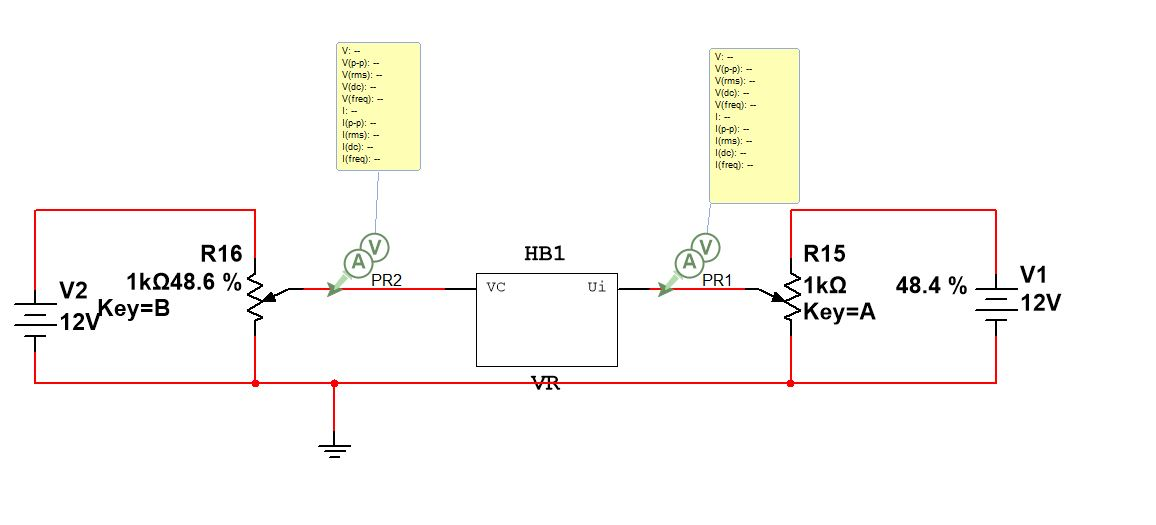
\includegraphics[width=\textwidth]{2.jpg}
\caption{直流工作情况分析}
\label{2}
\end{figure}

\begin{table}[h]
\centering
\caption{不同工作状态下对地电阻的关系}
\label{ttable}
\begin{tabular}{|c|c|c|c|c|c|c|}
\hline
$V_C$&$U_i=1\mathrm{V}$&$U_i=2\mathrm{V}$&$U_i=3\mathrm{V}$&$U_i=4\mathrm{V}$&$U_i=5\mathrm{V}$&$U_i=6\mathrm{V}$\\
\hline
1V&$13.3\mathrm{k}\Omega$&$11.9\mathrm{k}\Omega$&$11.9\mathrm{k}\Omega$&$11.9\mathrm{k}\Omega$&$12.0\mathrm{k}\Omega$&$12.1\mathrm{k}\Omega$\\
\hline
2V&$20.1\mathrm{k}\Omega$&$20.0\mathrm{k}\Omega$&$20.0\mathrm{k}\Omega$&$20.0\mathrm{k}\Omega$&$19.9\mathrm{k}\Omega$&$20.0\mathrm{k}\Omega$\\
\hline
3V&$30.0\mathrm{k}\Omega$&$30.0\mathrm{k}\Omega$&$29.9\mathrm{k}\Omega$&$30.1\mathrm{k}\Omega$&$29.9\mathrm{k}\Omega$&$30.1\mathrm{k}\Omega$\\
\hline
4V&$39.9\mathrm{k}\Omega$&$40.0\mathrm{k}\Omega$&$40.0\mathrm{k}\Omega$&$40.0\mathrm{k}\Omega$&$40.0\mathrm{k}\Omega$&$40.1\mathrm{k}\Omega$\\
\hline
5V&$49.8\mathrm{k}\Omega$&$50.0\mathrm{k}\Omega$&$50.0\mathrm{k}\Omega$&$50.1\mathrm{k}\Omega$&$49.9\mathrm{k}\Omega$&$50.0\mathrm{k}\Omega$\\
\hline
\end{tabular}

\begin{tabular}{|c|c|c|c|c|c|c|}
\hline
$V_C$&$U_i=7\mathrm{V}$&$U_i=8\mathrm{V}$&$U_i=9\mathrm{V}$&$U_i=10\mathrm{V}$&$U_i=11\mathrm{V}$&$U_i=12\mathrm{V}$\\
\hline
1V&$12.1\mathrm{k}\Omega$&$12.3\mathrm{k}\Omega$&$12.2\mathrm{k}\Omega$&$12.3\mathrm{k}\Omega$&$12.4\mathrm{k}\Omega$&$12.1\mathrm{k}\Omega$\\
\hline
2V&$20.2\mathrm{k}\Omega$&$20.4\mathrm{k}\Omega$&$20.3\mathrm{k}\Omega$&$20.2\mathrm{k}\Omega$&$20.1\mathrm{k}\Omega$&$20.0\mathrm{k}\Omega$\\
\hline
3V&$30.1\mathrm{k}\Omega$&$30.5\mathrm{k}\Omega$&$29.3\mathrm{k}\Omega$&$30.2\mathrm{k}\Omega$&$30.0\mathrm{k}\Omega$&$29.8\mathrm{k}\Omega$\\
\hline
4V&$39.7\mathrm{k}\Omega$&$40.2\mathrm{k}\Omega$&$40.5\mathrm{k}\Omega$&$40.1\mathrm{k}\Omega$&$40.3\mathrm{k}\Omega$&$40.2\mathrm{k}\Omega$\\
\hline
5V&$50.2\mathrm{k}\Omega$&$50.4\mathrm{k}\Omega$&$49.8\mathrm{k}\Omega$&$50.4\mathrm{k}\Omega$&$49.9\mathrm{k}\Omega$&$49.9\mathrm{k}\Omega$\\
\hline
\end{tabular}
\end{table}
从仿真数据中我们可以看到电阻对控制电压具有相当好的精确性,其中,$V_c=1\mathrm{V}$时误差较大的原因是回路的基本电阻为$10\mathrm{k}\Omega$,控制电阻希望达到$R_{Q_1}=0$的情况,而这是不可能的。

另外在仿真中发现部分时间可能出现仿真错误,可能和积分环节和电容有关,重新开始仿真之后发现问题得到了解决。

\subsection{交流情况仿真}
我们对交流情况做一个简单的仿真来验证电阻的性能。如图\ref{3}所示,我们输入5V峰峰值的电压,频率取10Hz,
测量压控电阻上的分压,如图\ref{4}所示。

\begin{figure}
\centering
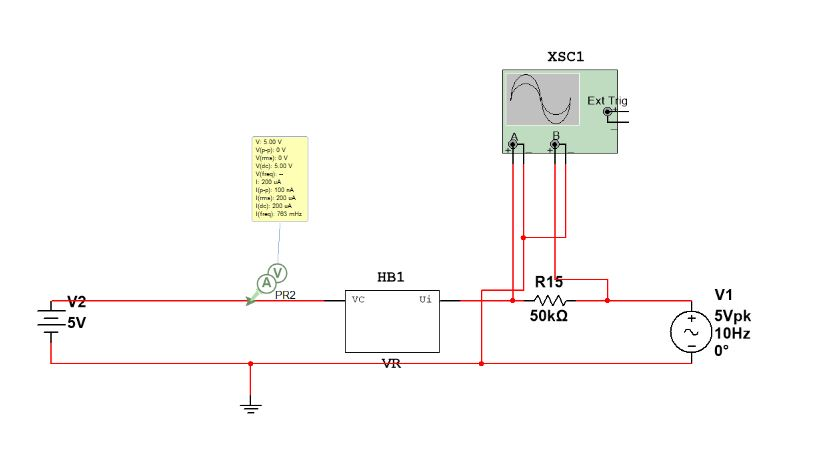
\includegraphics[width=\textwidth]{3.jpg}
\caption{交流情况仿真}
\label{3}
\end{figure}
\begin{figure}
\centering
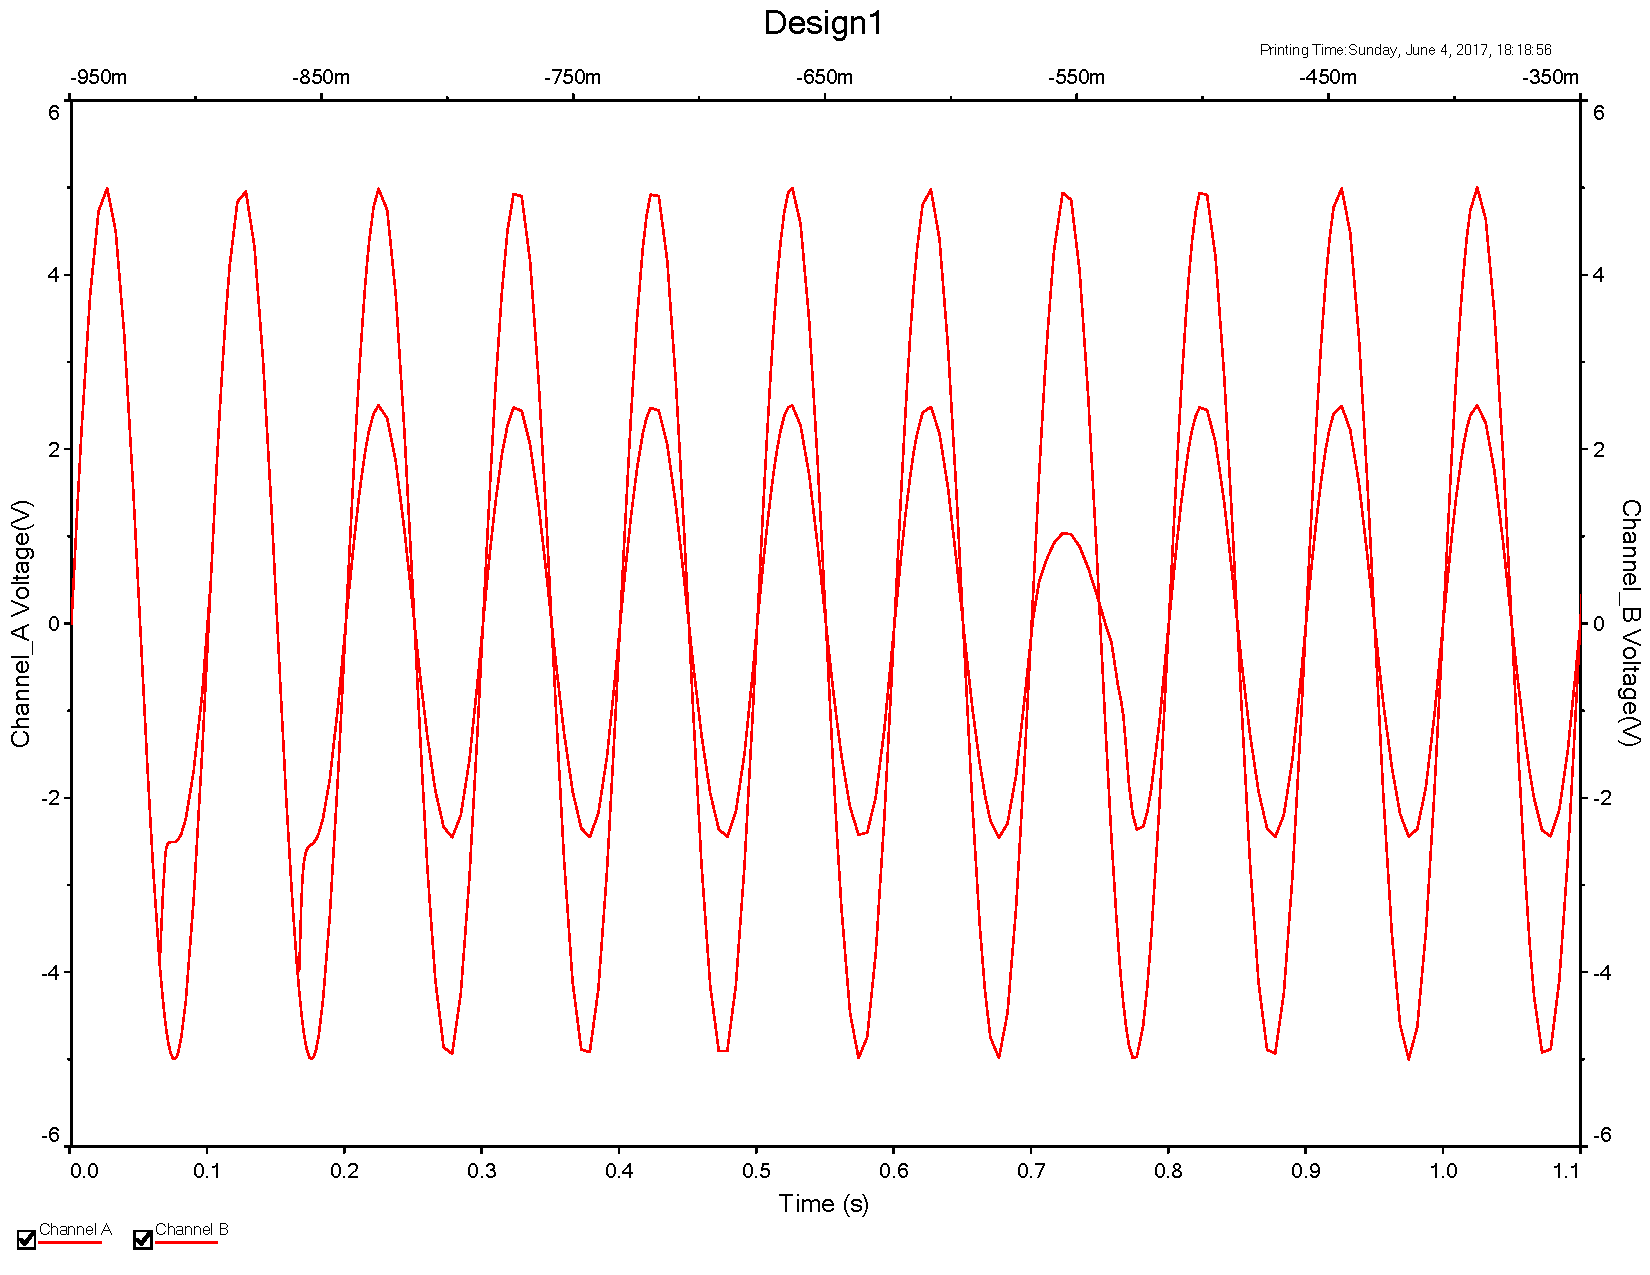
\includegraphics[width=\textwidth]{1.pdf}
\caption{交流情况仿真效果}
\label{4}
\end{figure}

从电路我们可以看出理想情况的分压应为整个分压的一半,但是我们可以看出,在电路开始运行的几个周期内,控制器没有达到稳态,因此,
如果进一步增加高频,可能控制器将无法正常工作(延迟时间远远大于信号周期)。同时也可以看出控制系统稳定之后系统的输出和理想情况相符,
并且没有额外的相位差。

通过仿真,我们可以看出电路的工作情况还是比较理想的,并且找出了所有影响电路正常工作的原因。

\section{电路优劣势分析}
\subsection{优势}
由模拟元件组成的电路,在造价上和ADDA式压控电阻相比具有明显的优势。整个电路仅采用了6个运放(相当于两个芯片),1个乘法器,同时,
电路中采取的所有电阻均是$10\mathrm{k}\Omega$,对于搭建和集成化提供了便利。同时可以看出,外围电路明显简化。线性性良好,并且可以
连续控制(相比于ADDA压控电阻控制精度取决于数模转换精度)
\subsection{劣势}
因为必须引入基准电阻,因此电路的最小阻值受限。另外,因为要引进1V的补偿标准电源,因此在集成上存在困难。当然,后者可以采取将1V标准电源
取消而将整个模块控制电压——电阻方程变为$R_{ui}=10V_C\mathrm{k}\Omega/\mathrm{V}+10\mathrm{k}\Omega$的增量线性方程。
\section{可以做的进一步调整}
受到时间限制,不能对电路进行进一步的调整,但是整个电路仍存在着很多可以调整的空间,例如
\begin{itemize}
\item 引入PID单元提高系统的响应速度

目前电路的反馈控制仅仅是最简单I单元,没有控制电路的响应速度和可能出现的震荡,对于这个电路,可以采取控制理论的方式进行校正,例如串联PID单元或反馈校正,提高系统的响应速度。

\item{选取合适的元件降低电路的基础电阻}

可以通过选取更合适的JFET和参数调整等方式确定更低的电路基础电阻$R_1$,使得电路有着更好的特性。

\item{三角波——正弦波转换}

在电路的响应速度达到要求之后,可以完成三角波——正弦波转换,具体方式是通过某种电路测量三角波的周期(显然,如果已知三角波波形,这种电路
很好设计)之后,将三角波的周期通过T-V模块转化成为电压,不妨我们记这个电压为$V_T=\alpha T$,其中$\alpha$为常数。之后通过此压控电阻
转化为电阻$R_F=\beta T$,(其中$\beta$为常数)并使用电阻——电容正弦波震荡网络输出频率为$f=\frac{\gamma}{T}$的正弦波信号,
只要电路参数设计的合理,完全可以使得$\gamma=1$使得生成同频率正弦波,完成相关的转化工作。并且相关电路的实现也比较简单

实际上,这一点也是本电路设计时的初衷和灵感的来源。

\end{itemize}

\end{document}